\section{Създаване на симулационна система}
	
	След анализът върху съществуващите симулационни системи изглежда, че
	система която да реши поставените проблеми, не съществува.
	Повечето от тях, имат примитивни \ac{GUI} които не предоставят
	необходимата гъвкавост на точно определена създадена за целта такава.
	
	Под голям въпрос е и качеството на документацията, както и състоянието на
	наличните примери и качество на кода. Това оставя възможността да бъде разгледан
	един нетрадиционен вариант за решаване на такъв проблем.

	\subsection{Модел}
	
		За създаването на нашият модел и цялостната програма ще се използва итеративен подход \cite{ArtOfAgile}.
		Това означава, че ще изградим основните части от системата - 
		първо\footnote{Посоченият подход е лична интерпретация}. Допълнителна 
		функционалност ще добавяме само, когато сме доволни от качеството на текущата програма. 
				
		Основната част от програмата ще контролира заложените закони и взаимодеиствия	между обектите.
		При всяка нова стъпка от симулацията, обектите участващи в нея ще предоставят информация за
		състоянието в което се намират. То може да се променя, като това е изразено в промяна
		на техните свойства.
		
		Необходимостта за изобразяване на самата симулация, по време на изпълнение и когато тя вече е приключила,
		води до някои допълнителни ограничения. Системата трябва да работи достатъчно бързо\footnote{Между 30 и 60 кадъра в секунда},
		за да предоставя гладка и лека работа за потребителя.
		
		С така поставените ограничения и подходи, използването на \ac{DES} предоставя:
		
		\begin{itemize}
			\item Гъвкавкост
			\item Лесна имплементация
			\item Лесна промяна
			\item Лесно скриване на детайлите от самия потребител			
		\end{itemize}				
		
		Още повече, за симулация на трафик е необходима симулация от тип опашка, която в повече от случаите
		се имплементира с помощта на \ac{DES} \cite{Barlas}.
		
		При стартиране на системата, тя ще изисква от потребителя да въведе необходимите данни за 
		стартиране на симулация. Когато тя започне, на потребителя се дава възможност визуално
		да наблюдава симулацията на всяка своя стъпка. След приключването й, се предоставят
		данни от протичане на симулацията.	На фиг. \ref{figure:systemModel} е изобразена диаграма, която показва
		работата на така зададения модел.	
		
		
		\begin{figure} 
				\caption{Модел на симулационната система}
				\label{figure:systemModel}
				\begin{center}
				
					\begin{tikzpicture}[scale=2, node distance = 4cm, auto]
					    % Place nodes
					    \node [start] (init) {Начало};
					    \node [block, below of=init, node distance = 4cm] (load-settings) {Зареждане на настройки};
					    \node [block, right of=load-settings, node distance = 5cm] (next-step) {Преминаване към следващо състояние};
					    \node [block, below of=next-step, node distance = 3cm] (draw-current-state) {Изобразяване на текущото състояние};
					    \node [decision, below of=draw-current-state, node distance = 5cm] (is-end) {Приключила ли е симулацията?};
					    \node [block, below of=is-end, node distance = 5cm] (results) {Показване на крайните резултати};
					    \node [exit, left of=results, node distance = 5cm] (end) {Край};
					    % Draw edges
					    \path [line] (init)               -- (load-settings);
					    \path [line] (load-settings)      -- (next-step);
					    \path [line] (next-step)          -- (draw-current-state);
					    \path [line] (draw-current-state) -- (is-end);
					    \path [line] (is-end.east)        |- node[above right] {Не} (next-step.east);
					    \path [line] (is-end)             -- node[midway] {Да} (results);
					    \path [line] (results)            -- (end);
					\end{tikzpicture}	
			
			\end{center}	
			
		\end{figure}						
		\newpage
	
	\subsection{Компоненти на симулацията}		
	\subsection{Избор на технология и програмен език}
		\subsubsection{Света на Lua}
		
			Lua е малък скриптов език, който кара да се усмихнеш, когато го използваш. 
			Според авторите му той е: \footnote{\url{http://www.lua.org/about.html}} 
			
			\begin{itemize}
				\item Бърз
				\item Лек
				\item Лесен за вграджане (embeddable)
				\item Доказан
			\end{itemize}
			
			Той е напълно безплатен за употреба. Разпространява се под 
			\emph{MIT}\footnote{\url{http://www.opensource.org/licenses/mit-license.php}} лиценз. 
			Доказал се е като добър избор за скриптов език за множество комерсиални 
			игри\footnote{\url{http://en.wikipedia.org/wiki/Category:Lua-scripted_video_games}}.
			
			Автори на езика са Roberto Ierusalimschy, Waldemar Celes и Luiz Henrique de Figueiredo. Те разработват езика в
			университета PUC-Rio\footnote{\url{http://www.puc-rio.br/index.html}}, като част от нуждите за тяхната група
			от технологии за компютърна графика. 
			
			Името на езика идва от португалската дума Lua, която означава ``Луна``.
			
			Lua е смесица между обектно-ориентиран, функционален и програмиране свързано с данни (data-driven development)
			подход към създаването на програми. Има лесен за научаване синтаксис и сравнително малък брой концепции. 
			
			Имплементиран е като библиотека за програмния език \emph{C}\footnote{\url{http://en.wikipedia.org/wiki/C_(programming_language)}}. 
			Поради тази причина, той няма концепция за``основна програма`` (main program). Нуждае се от приемник (host), който извиква различни
			части от код, написан на \emph{Lua}.
			
			С помощта на \emph{C} функции, \emph{Lua} може да бъде пригоден за работа в различни, непредвидени от авторите му,
			области и споделя вече съществуващия синтаксис.
			
			\emphparagraph{Концепции}
				Lua е динамично типизиран език (dynamically typed), което означава, че само стойностите имат тип.
				
				\lstinputlisting[title=Променливи]{code/lua/variables.lua}				
				\lstinputlisting[title=Изход]{code/lua/variables.output}
				
				Има концепция за прихващане на грешките, която много се доближава до тази на изключенията от езици като
				C++ и Java.
				
				\lstinputlisting[title=Грешки]{code/lua/errors.lua}
				\lstinputlisting[title=Изход]{code/lua/errors.output}
				
				\newpage
				
				Езикът предоставя и съвместни програми (coroutines). Съвместна програма в Lua представлява изпълнение на независима нишка.
				
				\lstinputlisting[title=Съвместни програми]{code/lua/coroutines.lua}
				
				\lstinputlisting[title=Изход]{code/lua/coroutines.output}
				
				\newpage
				
				Използването на класове в \emph{Lua} е малко по-интересно и странно, в сравнение с езици като \emph{C} и \emph{Java}. 
				То по-скоро напомня на прототипното наследяване в
				\emph{JavaScript}\footnote{\url{http://www.crockford.com/javascript/inheritance.html}}.
				Това позволява на всеки разработчик да създаде свой, собствен стил на писане на класове. Това може да е добро и лошо нещо.
				
				\lstinputlisting[title=Класове]{code/lua/classes.lua}
				
				\lstinputlisting[title=Изход]{code/lua/classes.output}				
		
		\subsubsection{Нужда от по-висока абстракция}
		
			Lua е прекрасен малък език, но сам по себе си, той не доставя необходимите инструменти
			за лесно създаване на симулационна система. Намиране на библиотека предоставяща по-висока
			абстракция е задължително.
			
			Една такава библиотека е \emph{Moai}\footnote{\url{http://getmoai.com/}} (произнася се Moe-Eye).
			Тя е по-скоро двигател за игри (game engine).
			Разработката й е започнала през 2010г. и е активно разработвана и до днес. 
			Тя е с \emph{отворен код}\footnote{\url{http://github.com/moai/moai-dev}}
			и използва лицензът \emph{CPAL}\footnote{\url{http://www.opensource.org/licenses/cpal_1.0}}, който
			позволява да използваме софтуера за нашите цели. 
			Разработена е от \emph{Zipline Games}\footnote{\url{http://www.ziplinegames.com/}}.						
			
			\emph{Moai} е библиотека за разработване на игри върху множество от платформи, вариращи от десктоп до
			мобилни операционни системи. За основна графична библиотека се използва стандартът 
			\emph{OpenGL}\footnote{\url{http://www.opengl.org/}}, който позволява тази разнообразност.
			Поради добрата си свързаност със \emph{C}, Moai може да постигне производителност, по-висока
			от тази на приложения написани на  \emph{Objective C}
			\footnote{\url{http://en.wikipedia.org/wiki/Objective-C}} за \emph{iPhone}.

			Обеткният модел на \emph{Moai} е изцяло написан на \emph{C++} и използва префикс ``MOAI``. Тези обекти
			се изчистват от \ac{GC}, също както и тези в \emph{Lua}. За това спомагат и т.нар. контейнери в \emph{Moai},
			които се грижат да не останат неизчистени обекти от паметта.
			
			\newpage			
			
			Програма, изписваща на екрана ``Hello from Moai``, излежда така:
			
			\lstinputlisting[title=Здравей Moai]{code/moai/hello-moai.lua}			
			
			Когато програмата се изпълни, на екрана се визуализира фиг. \ref{figure:hello-moai}
			
			\begin{figure} 
				\caption{Резултат изпълнението на първата програма на \emph{Moai}}
				\label{figure:hello-moai}
					\begin{center}
						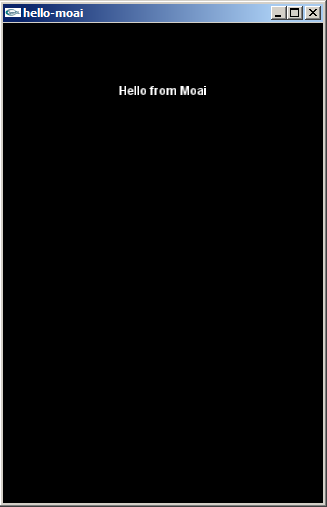
\includegraphics{assets/images/hello-moai.png}				
					\end{center}
			\end{figure}
			
			\newpage

			
	\subsection{Програмиране на системата}